% tikzpic.tex
\documentclass[preview,tikz]{standalone}% 'crop' is the default for v1.0, before it was 'preview'
%\usetikzlibrary{...}% tikz package already loaded by 'tikz' option
\usetikzlibrary{arrows,shapes,backgrounds}
\begin{document}
\tikzstyle{background grid}=[draw, blue!30,step=.5cm,very thin]
	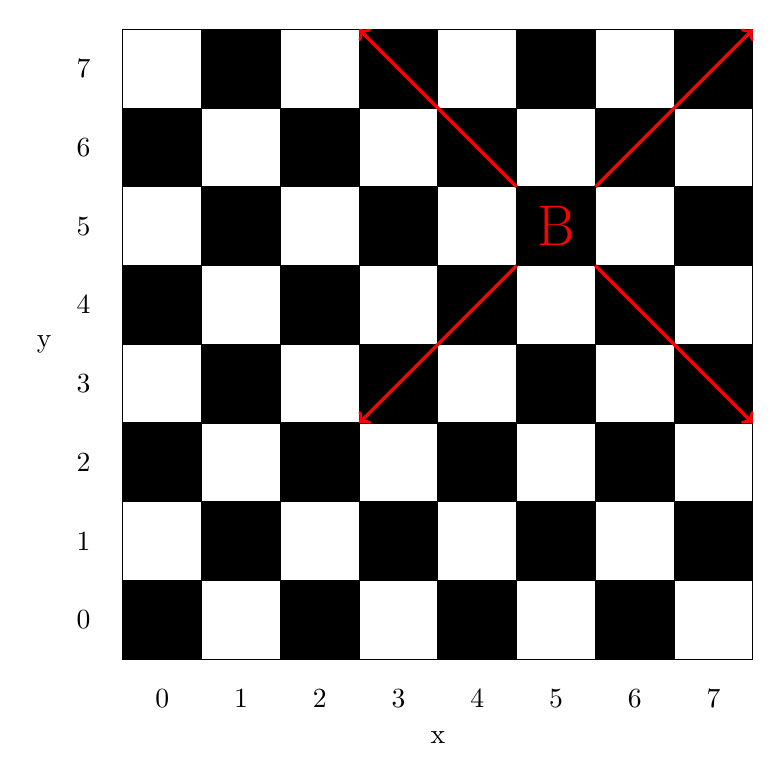
\begin{tikzpicture}[x=1cm]
		\foreach \y in {0,2,...,6}{
			\foreach \x in {0,2,...,6}{
				\draw[fill=black] (\x,\y) rectangle (1+\x,1+\y) rectangle (2+\x,2+\y);
				\draw[] (\x, 2+\y) rectangle (\x+1, \y+1) rectangle (2+\x, \y);
			}
		}
		
		\foreach \x in {0,1,...,7}{
			\node() at (\x+0.5, -0.5) {\x};
		}
		\node() at (4,-1){x};
		\foreach \x in {0,1,...,7}{
			\node() at (-0.5, \x+0.5) {\x};
		}
		\node() at (-1,4){y};		
		\node[anchor=center, red] at (5.5,5.5) {\huge{B}};
		\draw[very thick, red, ->] (5,5) -- (3,3);
		\draw[very thick, red,->] (6,6) -- (8,8);	
		\draw[very thick, red,->] (5,6) -- (3,8);
		\draw[very thick, red,->] (6,5) -- (8,3);
	\end{tikzpicture}
	
\end{document}
